\chapter{Grundlagen}
Um den Mikrocontroller zu implementieren, der Tastatureingabesequenzen sowohl aufnehmen als auch wiedergeben soll, müssen dafür einige Grundlagen benannt werden. Dieses Kapitel beschreibt im Folgenden die benötigten Elemente der PS/2-Tastaturschnittstelle und des PS/2-Protokolls, sowie einige verwandte Arbeiten in dieses Themengebiets als auch die rechtlichen Grundlagen. Die Abschnitte PS/2-Tastaturschnittstelle und PS/2-Protokoll fassen die Beschreibungen von Adam Chapweske \cite{chapweske} bzw. der Übersetzung von Bernward Mock \cite{mock} zusammen.



\section{PS/2-Tastaturschnittstelle}
IBM entwickelte 1987 die PS/2-Tastatur zur Verwendung am gleichnamigen PC, dem Personal System/2, und ist kompatibel mit der zuvor entwickelten AT-Tastatur. Der Anschluss erfolgt über einen 5- oder 6-poligen Mini-DIN Stecker, bzw. alternativ über einen SDL-Stecker. In Abbildung \ref{female_pins} \cite{female_pins} ist die Anordnung der 6 Pins aufseiten des PCs (female) zu sehen. Spiegelverkehrt dazu ist der Anschluss der Tastatur (male).

\begin{figure}
  \centering
  \begin{minipage}{0.45\textwidth}
    \centering
    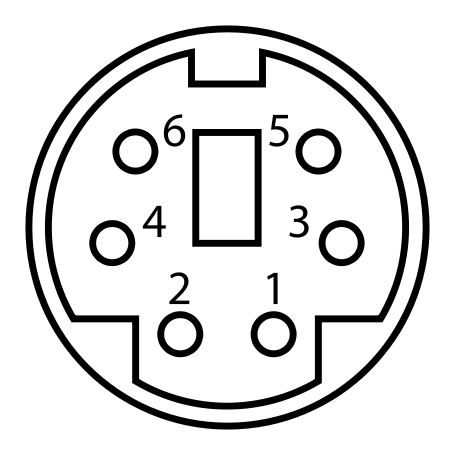
\includegraphics[width=0.48\linewidth]{images/female_pins.png}
    \caption{PS/2 Female Pins}
    \label{female_pins}
  \end{minipage}
  \begin{minipage}{0.45\textwidth}
    \centering
    \begin{tabular}{|l|l|} \hline
      Pin 1 & Daten \\ \hline
      Pin 2 & kein Signal \\ \hline
      Pin 3 & Erdung \\ \hline
      Pin 4 & 5 Volt \\ \hline
      Pin 5 & Takt \\ \hline
      Pin 6 & kein Signal \\ \hline
    \end{tabular}
    \caption{Pin Spezifikation}
    \label{pin_specification}
  \end{minipage}
\end{figure}

Für die Verwendung einer PS/2-Tastatur werden nur 4 der 6 Pins benötigt, da ein Datensignal, eine Erdung, ein Takt und eine Leitung mit 5 Volt ausreichen um Tastensignale zu übertragen (siehe Abbildung \ref{pin_specification}). Ein in der Tastatur verbauter Mikrocontroller, ein sogenannter Keyboard-Encoder, scannt die Tasten und überprüft ob eine Taste gedrückt ist oder nicht. PS/2-Tastaturen verwenden typischerweise zwischen 84 bis 104 Tasten, welche sogenannten Scancodes zugeordnet werden. Es existieren drei Scancode-Sets, wobei PS/2-Tastaturen den als Scancode-Set 2 bekannten Satz benutzen. In Abbildung \ref{scancodes} \cite{scancodes} ist ein Ausschnitt dieser Scancodes auf einigen Tasten zu sehen und im Anhang befindet sich die Tabelle \ref{scancode_set_2} des gesamten Scancode-Sets 2.

\begin{figure}
  \centering
  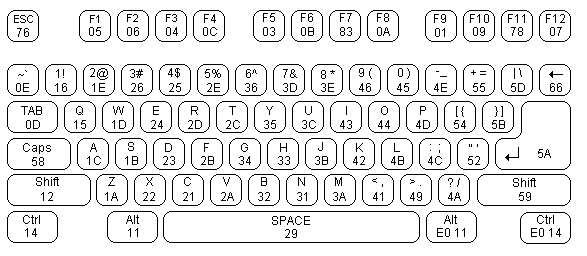
\includegraphics[width=0.9\textwidth]{images/scancodes.jpg}
  \caption{Scancode-Set 2 Ausschnitt}
  \label{scancodes}
\end{figure}

Die Scancodes sind Hexadezimalwerte bestehend aus einem Makecode, welcher gesendet wird wenn die Taste gedrückt wird, und einem Breakcode, der beim Loslassen der Taste gesendet wird. Breakcodes setzen sich in fast allen Fällen aus einem 0xf0 und dem Makecode der Taste zusammen. Zudem existieren erweiterete Tasten, deren Makecode länger als ein Byte ist und zusätzlich ein 0xe0 als erstes Byte haben, was auch für den zugehörigen Breakcode gilt. Um also z.B. ein ``G'' wiederzugeben ist es notwendig zuerst die Shift-Taste gedrückt zu halten, die G-Taste zu drücken und beide Tasten in umgekehrter Reihenfolge loszulassen. Dementsprechend können für dieses Beispiel die folgenden Scancodes übertragen werden: 0x12 (Make L Shift), 0x34 (Make G), 0xf0 0x34 (Break G) und 0xf0 0x12 (Break L Shift).

Wenn eine Taste dauerhaft gedrückt wird setzt die Wiederholfunktion des Mikrocontrollers der Tastatur ein, auch Typematic genannt. Diese sendet mit einer gewissen Verzögerung (typematic delay) den Makecode der zuletzt gedrückten Taste und dann mit einer bestimmten Wiederholrate (typematic rate) fortwährend denselben Makecode, bis die Taste losgelassen wird. Beide Parameter können durch den PC, in diesem Zusammenhang auch Host genannt, eingestellt werden, wobei die Verzögerung zwischen 0,25 und 1,00 Sekunden liegen kann und die Wiederholrate zwischen 2,0 cps und 30,0 cps (Zeichen pro Sekunde).

Die Tastatur kann weiterhin einen Reset vollziehen und führt dabei einen Selbsttest, auch Basic Assurance Test (BAT) genannt, durch. Dabei wird die Verzögerung auf 0,5 Sekunden und die Wiederholrate auf 10,9 cps gesetzt, sowie Scancode-Set 2 geladen. Zudem werden zu Beginn des BAT die drei LEDs der Tastatur an und danach wieder ausgeschaltet, sowie 0xaa an den Host gesendet für ein erfolgreich abgeschlossenen BAT.

Die Kommunikation zwischen dem Host und der Tastatur wird im folgenden Abschnitt anhand des PS/2-Protokolls beschrieben.



\section{PS/2-Protokoll}
Bei dem PS/2-Protokoll handelt es sich um ein sogenanntes bi-direktionales serielles Protokoll. Dies bedeutet, dass auch der Host Befehle an die Tastatur senden kann, im Fall des PS/2-Protokolls sind es 17 Host-Befehle. Eine detaillierte Auflistung dieser Befehle zeigt die Tabelle ... im Anhang.
\begin{figure}
  \centering
  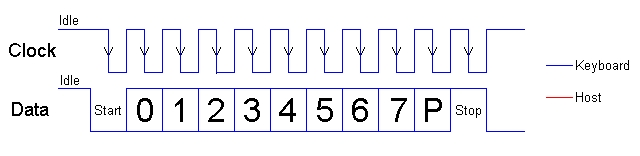
\includegraphics[width=1\textwidth]{images/device_to_host.jpg}
  \caption{Kommunikation Tastatur zu Host}
  \label{device_to_host}
\end{figure}
1 Startbit, immer 0
8 Datenbits mit LSB voran
1 Parity-Bit (ungerade Parität)
1 Stopbit, immer 1
ggf. 1 ACK-Bit (nur bei Host zu Tastatur)



\section{Verwandte Arbeiten}
Wie bereits in der Einleitung erwähnt, existieren viele Produkte im Bereich der Hardware-Keylogger. So gibt es bereits Keylogger für USB-Tastaturen und PS/2-Tastaturen mit verschiedenen Speichergrößen oder der Möglichkeit die aufgezeichneten Tastatureingaben über Wi-Fi zu versenden \cite{keelog}.

Im Bereich der Mikrocontroller gibt es verschiedene Bibliotheken, die das Mitlesen von Tastatureingaben ermöglichen. Eine verbreitete Implementierung ist eine Bibliothek, die sowohl für Arduino Mikrocontroller als auch andere Mikrocontroller gedacht ist \cite{ps2keyboard}. Die bereitgestellten Funktionen erlauben es, wie in den mitgelieferten Beispielen gezeigt wird, die Tastatureingaben der mit dem Mikrocontroller verbundenen Tastatur über den Mikrocontroller auszugeben. Auch in anderen Implementierungen, wie z.B. dem Tastaturtreiber des Betriebssystems PrettyOS, werden Tastatureingaben entgegen genommen und in ASCII-Zeichen umgewandelt, um diese u.a. auf dem Bildschirm auszugeben \cite{prettyos}.

Es wurden aber auch Konzepte und deren Umsetzung dokumentiert, welche die Manipulation von Tastatureingaben zeigen. In einem bestehenden Ansatz wurde die Firmware des Mikrocontrollers einer Apple-Tastatur überschrieben \cite{chen}. Dies hatte zur Folge, dass nach einer normalen Zeicheneingabe und einer bestimmten Befehlsequenz diese Zeicheneingabe erneut, aber spiegelverkehrt an den PC gesendet wurde.

Andere Ansätze werden zudem als Produkt vertrieben, wie z.B. der USB-Stick Rubber Ducky \cite{ducky}. Dieser enthält unter seiner Abdeckung einen zusätzlichen Mikrocontroller mit einer Speicherkarte. Mithilfe von eigenen Befehlen, die in einer Textdatei auf der Speicherkarte gespeichert werden kann, führt der USB-Stick diese Befehle als Tastatureingaben aus, sobald er mit einem PC verbunden wird.

Zuletzt wurde ein weiterer Ansatz präsentiert, welcher BadUSB \cite{badusb},

Der Unterschied zu dem Ansatz dieser Bachelorarbeit besteht darin, dass für die Wiedergabe von Tastatureingabesequenzen nicht der Mikrocontroller der Tastatur angepasst werden soll. Stattdessen wird ein eigener Mikroccontroller die Tastatureingaben tätigen, die vorher dem Mikrocontroller entweder via SD-Karte oder Ethernet übergeben wurden.



\section{Rechtliche Grundlagen}
Die rechtlichen Grundlagen für den Einsatz technischer Hilfsmittel zum unbefugten Aufzeichnen oder Manipulieren von Daten sind differenziert zu betrachten, denn meist ist die Rechtmäßigkeit einer Verwendung fallbezogen. Der Paragraph \S 202a Strafgesetzbuch \cite{stgb} regelt den unbefugten Zugriff auf Daten folgendermaßen:
\begin{quote}
  (1) Wer unbefugt sich oder einem anderen Zugang zu Daten, die nicht für ihn bestimmt und die gegen unberechtigten Zugang besonders gesichert sind, unter Überwindung der Zugangssicherung verschafft, wird mit Freiheitsstrafe bis zu drei Jahren oder mit Geldstrafe bestraft. \\
  (2) Daten im Sinne des Absatzes 1 sind nur solche, die elektronisch, magnetisch oder sonst nicht unmittelbar wahrnehmbar gespeichert sind oder übermittelt werden.
\end{quote}
Dies bedeutet zum Bespiel, dass es verboten ist mithilfe eines Hardware-Keyloggers die Tastatureingaben einer anderen Person unbefugt aufzuzeichnen.

Auch einem Arbeitgeber ist es im Allgemeinen nicht gestattet, Daten der Arbeitnehmer ohne deren Wissen festzuhalten \cite{bildscharbv}. Darüber hinaus regelt das Betriebsverfassungsgesetz, dass der Betriebsrat bei der Einführung technischer Hilfsmittel zur Aufzeichnung von Verhalten und Leistung der Arbeitnehmer Mitbestimmungsrechte besitzt \cite{betrvg}.

Anders verhält es sich beim Einsatz technischer Hilfsmittel zum Aufzeichnen von Daten bzgl. der Strafverfolgung. Zwar ist \S 100h Abs. 1 Nr. 2 Strafprozessordnung \cite{stpo} laut einer internen Einschätzung der Generalstaatsanwaltschaft München \cite{munich} nicht ausreichend, jedoch wurde mit \S 20k BKA-Gesetz \cite{bkag} entsprechende Grundlagen für den Einsatz solcher Hilfsmittel geschaffen. Somit ist z.B. der Einsatz von ``Remote Forensic Software'' (ugs. ``Bundestrojaner'') unter bestimmten Umständen möglich, welcher eine Funktion zur Aufzeichnung von Tastatureingaben besitzt \cite{spd}.